%\documentclass[a4paper]{article}
%\usepackage{beamerarticle}

\documentclass[ignorenonframetext]{beamer}
\usepackage{beamerthemesplit}
\usepackage{amssymb}

\usepackage{../fhnw-beamer}
\usepackage{fancyvrb}
\usepackage{hyperref}
\hypersetup{
    colorlinks=true,
    linkcolor=blue,
    filecolor=magenta,      
    urlcolor=cyan,
}
\urlstyle{same}

%\mode<article>{\usepackage{fullpage}}
%\mode<presentation>{\usetheme{Berlin}}

\date{\today}
\author{rolf.schmutz@fhnw.ch}
\institute{FHNW}
\title{Netzwerke und Kommunikation\\B-LS-MI 004\\Basisdienste\\DNS Verzeichnisdienst}


\begin{document} % ===============================================================

\section{NDK 02-050: DNS}



\begin{frame}
\titlepage
\end{frame}



\begin{frame}
\frametitle{Ziele}
\begin{itemize}
	\item{Sie kennen die Aufgaben von DNS}
	\item{Sie kennen die Funktionsweise von DNS}
	\item{Sie k\"onnen gezielt DNS-Server abfragen}
\end{itemize}
\end{frame}



\begin{frame}
\frametitle{DNS: Domain Name System}
\begin{itemize}
	\item{\begin{Huge}\texttt{http://www.eff.org/}\end{Huge}}
	\item{\begin{Huge}\texttt{ping www.google.com}\end{Huge}}
	\item{\begin{Huge}\texttt{mailto: president@whitehouse.gov}\end{Huge}}
	\item{\begin{Huge}\texttt{telnet kremvax.kreml.ru}\end{Huge}}
\end{itemize}
\begin{block}{Hostnamen}
$\rightarrow$ Menschen\footnote{und auch Programme$\ldots$} arbeiten lieber mit {\em (Host-, Domain-) Namen} als mit IP-Adressen\ldots $\rightarrow$ wir brauchen ein \em{Telefonbuch}
\end{block}
\end{frame}

\begin{frame}
\frametitle{DNS: Grundlage}
\begin{itemize}
  \item{IP arbeitet {\em nur} mit {\em IP-Adressen} und kennt keine {\em Host/Domainnamen}}
  \item{das entspricht genau dem Telefonnetz wo Nummern zu Namen auch zuerst im Telefonbuch nachgeschlagen werden m\"ussen}
  \item{genau wie beim Telefonnetz braucht IP keinen DNS/Verzeichnisdienst -- der dient nur zur vereinfachten Handhabung f\"ur Menschen und/oder Programme}
\end{itemize}
\end{frame}

\begin{frame}
\frametitle{DNS: $\ldots$die Zeit {\em vor}{ }\footnote{in der {\em Steinzeit}: vor 1983} DNS}
\begin{itemize}
	\item{SRI\footnote{Standford Research Institute: beteiligt an der Entwicklung des Internet} verwaltete eine zentrale \texttt{HOSTS.TXT} Datei mit Namen$\leftrightarrow$IP-Adressen}
	\item{der {\em Namensraum}{}\footnote{namespace} war {\em flach}, d.h. nur eine Ebene von Namen m\"oglich}
	\item{\"Anderungen mussten an SRI geschickt werden}
	\item{alle ``Kunden'' mussten regelm\"assig eine Kopie der Daten erstellen}
\end{itemize}
Nachteile:
\begin{itemize}
	\item{Last und Datenverkehr auf dem zentralen Server}
	\item{{\em Single point of failure}, alles h\"angt von einem Server ab}
	\item{Konsistenz: \"Anderungen waren nicht gleichzeitig bei allen ``Kunden'' sichtbar}
	\item{{\em Name clash}, jeder Name musste sorgf\"altig ausgew\"ahlt werden um Kollisionen zu verhindern}
	\item{exponentielles Wachstum der Datei}
\end{itemize}
\end{frame}


\begin{frame}
\frametitle{DNS: Factlets}
\begin{itemize}
	\item{DNS ist das {\em Domain Name System}, ein spezialisierter Verzeichnisdienst}
	\item{klassisches Client-/Server-Konzept mit UDP\footnote{``Telegramm''}}
	\item{Definiert in STD13, RFC1034, RFC1035 und {\em viele} zus\"atzliche RFCs}
	\item{h\"aufigste Anwendung: IP$\leftrightarrow$Hostname Verzeichnis}
	\item{{\em hierarchisch}{}\footnote{wie die ``alten'' Telefonb\"ucher mit Vorwahl, Ortskreis, etc} aufgebaut mit {\em Delegationen} von {\em subtrees} (subdomains, Unterb\"aumen)}
	\item{{\em verteilte} Datenbank: eine Ebene der Daten wird von einer Partei verwaltet. Kein Server kennt den gesamten Namensraum}
	\item{{\em Replikation}{}\footnote{synchronisierte Kopien} der Daten vom {\em Master} auf {\em Slave} Server\footnote{alte Bezeichnungen: {\em primary} und {\em secondaries}}}
	\item{Kommuniziert \"uber UDP f\"ur normale Anfragen und \"uber TCP f\"ur Replikation}
\end{itemize}
\begin{small}
\begin{block}{DNS}
$\rightarrow$ scalable, reliable and flexible: Skalierbar, zuverl\"assig und Erweiterungsf\"ahig
\end{block}
\end{small}
\end{frame}

\begin{frame}
\frametitle{DNS: hierarchischer Namensraum}
\begin{itemize}
	\item{der {\em Namenspfad} wird von den Bl\"attern (leaves) her ausgelesen: \texttt{www.ai.mit.edu} \begin{tiny}(``most-specific'' zu ``least-specific'', vergleichen Sie das mit Windows oder UNIX Filesystemen)\end{tiny}}
	\item{der vollst\"andige Pfadname, {\em FQDN} (fully-qualified-domain-name) und der relative Name {\em RDN} (relative-domain-name) entsprechen einem Pfad- und einem Dateinamen}
\end{itemize}
\vspace{0.5cm}
\hspace{-0.4cm}
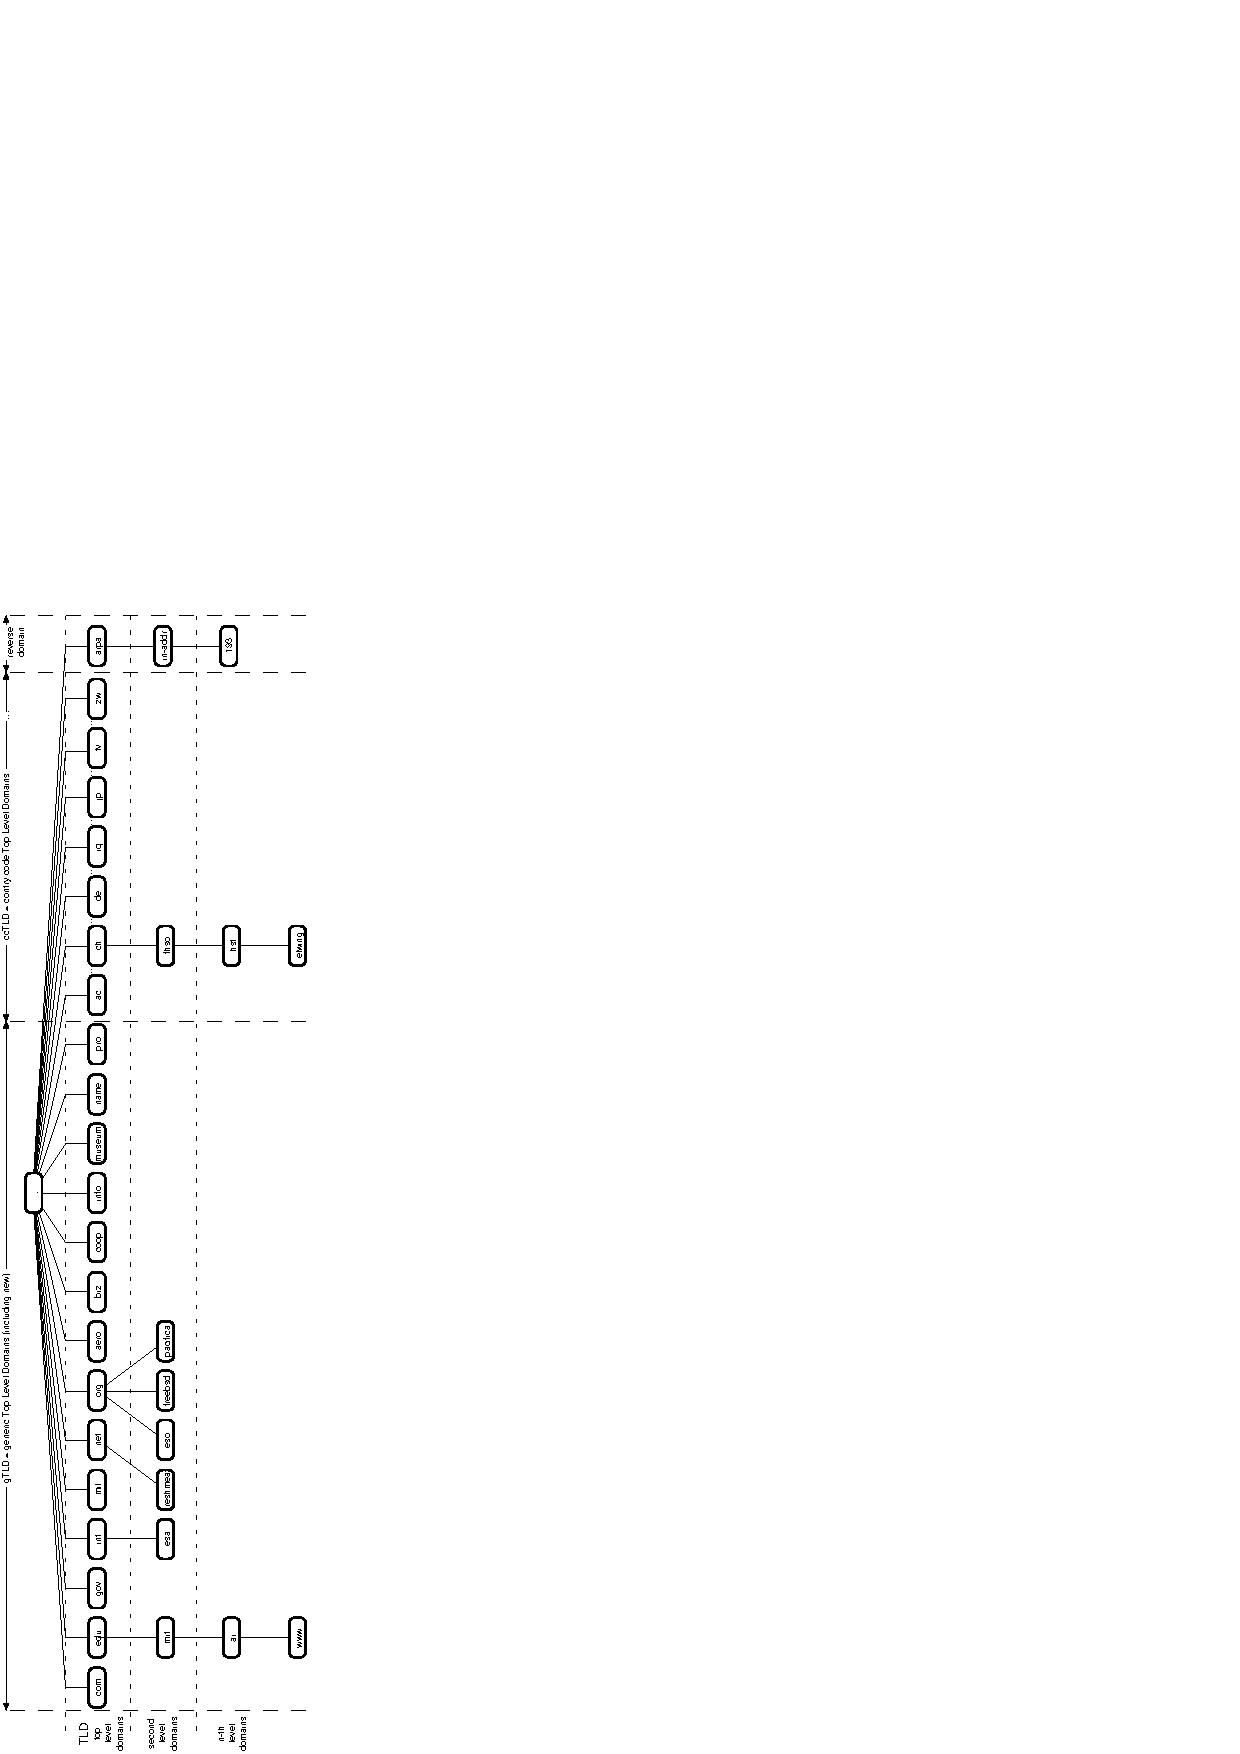
\includegraphics[width=18cm]{dns-hierarchy}
\end{frame}

\begin{frame}
\frametitle{DNS: Traditionelle Top-level Domains}
\begin{itemize}
	\item{gTLDs (generic top-level domain):\\ \begin{tabular}{rl}
	\texttt{com} & International: Kommerzielle Unternehmen: \texttt{www.sun.com} \\
	\texttt{edu} & USA: (Hoch-) Schulen (educational): \texttt{www.mit.edu} \\
	\texttt{gov} & USA: Regierung (governement): \texttt{www.whitehouse.gov} \\
	\texttt{int} & Internationale Organisationen: \texttt{www.esa.int} \\
	\texttt{mil} & USA: Milit\"ar: \texttt{www.norad.mil} \\
	\texttt{net} & International: Netzbetreiber/Infrastruktur: \texttt{www.sprint.net} \\
	\texttt{org} & International: Nichtkommerzielle Organisationen: \texttt{www.eff.org} \\
	\end{tabular}}
	\item{Reverse: IP-zu-Hostnamen\footnote{siehe Slide \ref{reverse}}: \texttt{67.242.135.193.in-addr.arpa}}
  \item{ccTLDs: country-code TLD: ISO-Code l\"anderspezifische Domains: \texttt{ch}, \texttt{de}, \texttt{us}, \texttt{tv}, \texttt{jp}, \texttt{to}, \texttt{tv}, \texttt{io}, \ldots}
\end{itemize}
\end{frame}

\begin{frame}\label{icann}
\frametitle{DNS: \href{https://www.icann.org/}{ICANN} neue Top-Level Domains}
Seit 2011 werden von ICANN (fast) beliebige Top-Level-Domains\footnote{wie .com, .org, .ch, \ldots} erteilt\footnote{f\"ur mindestens 1 Million \$US}.

\begin{itemize}
  \item Insbesondere wurden auch viele \href{https://en.wikipedia.org/wiki/Internationalized_domain_name}{IDN}\footnote{Internationalized Domain Names} neu geschaffen\footnote{vorallem Chinesische}
  \item Dies hat zu einem oft kritisierten Wildwuchs gef\"uhrt, mit mittlerweilen\footnote{2020}
1509 Top-Level-Domains (\href{https://data.iana.org/TLD/tlds-alpha-by-domain.txt}{Liste}).
  \item Gerade grosse Firmen mit dem Bed\"urfnis ihren Namen auf allen Top-Level-Domains
zu registrieren haben dagegen protestiert
\end{itemize}
\end{frame}


\begin{frame}\label{reverse}
\frametitle{DNS: Reverse Domain}
\begin{itemize}
	\item{f\"ur Abfragen von IP-Adresse $\rightarrow$ Domainname wird eine spezielle TLD \texttt{in-addr.arpa}{}\footnote{vom fr\"uheren ARPA-net -- es sind keine anderen Subdomains ausser \texttt{in-addr} mehr vorhanden} verwendet}
	\item{die Namen werden ebenfalls von den Bl\"attern (unten) her ausgelesen -- deshalb wird eine IP-Adresse ``verkehrt herum'' dargestellt: \texttt{www.fhnw.ch} $\rightarrow$ \texttt{50.3.86.147.in-addr.arpa}}
\end{itemize}
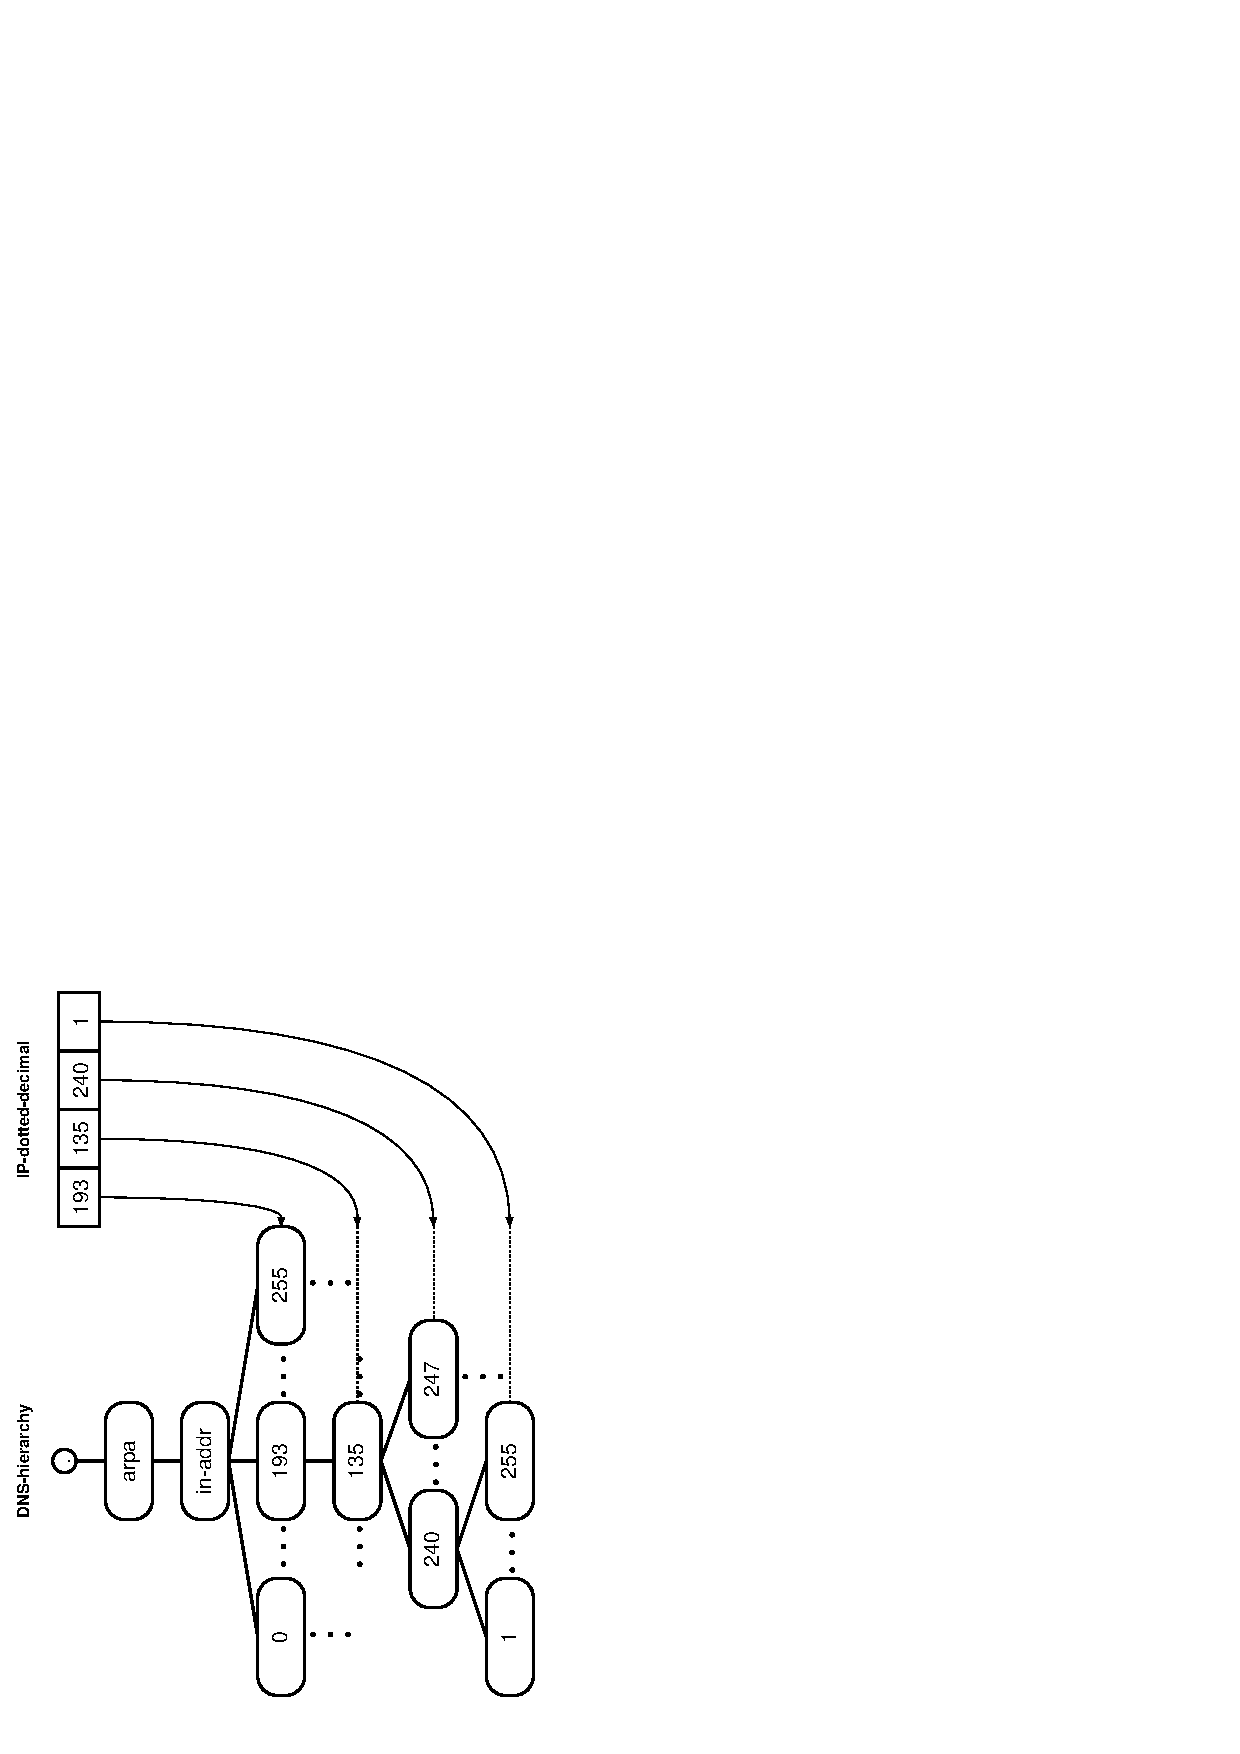
\includegraphics[width=12cm]{dns-reversehierarchy}
\end{frame}




\begin{frame}
\frametitle{DNS: Verteilte Datenbasis, Zonen und Delegation}
\begin{itemize}
	\item{die Verwaltung {\em authority} \"uber einzelne Teilb\"aume (subtree/domain) wird {\em delegiert} \begin{tiny}(per NS-record, der Verwalter ist zust\"andig f\"ur die Daten und die korrekte Funktion der Server)\end{tiny}}
	\item{die Daten werden in {\em Zonen} \begin{tiny}(entspricht einer Verzeichnisebene im Filesystem)\end{tiny} aufgeteilt und sind deshalb nicht mehr zentral verwaltet}
	\item{die {\em skalierung} (Wachstum) dieses Systems ist fast unbegrenzt m\"oglich}
	\item{ein Teilbaum {\em subtree} wird als {\em Domain} bezeichnet}
	\item{eine Verzeichnisebene wird als {\em Zone} bezeichnet und wird \"ublicherweise in einer Datei auf dem Server abgelegt}
\end{itemize}
\begin{center}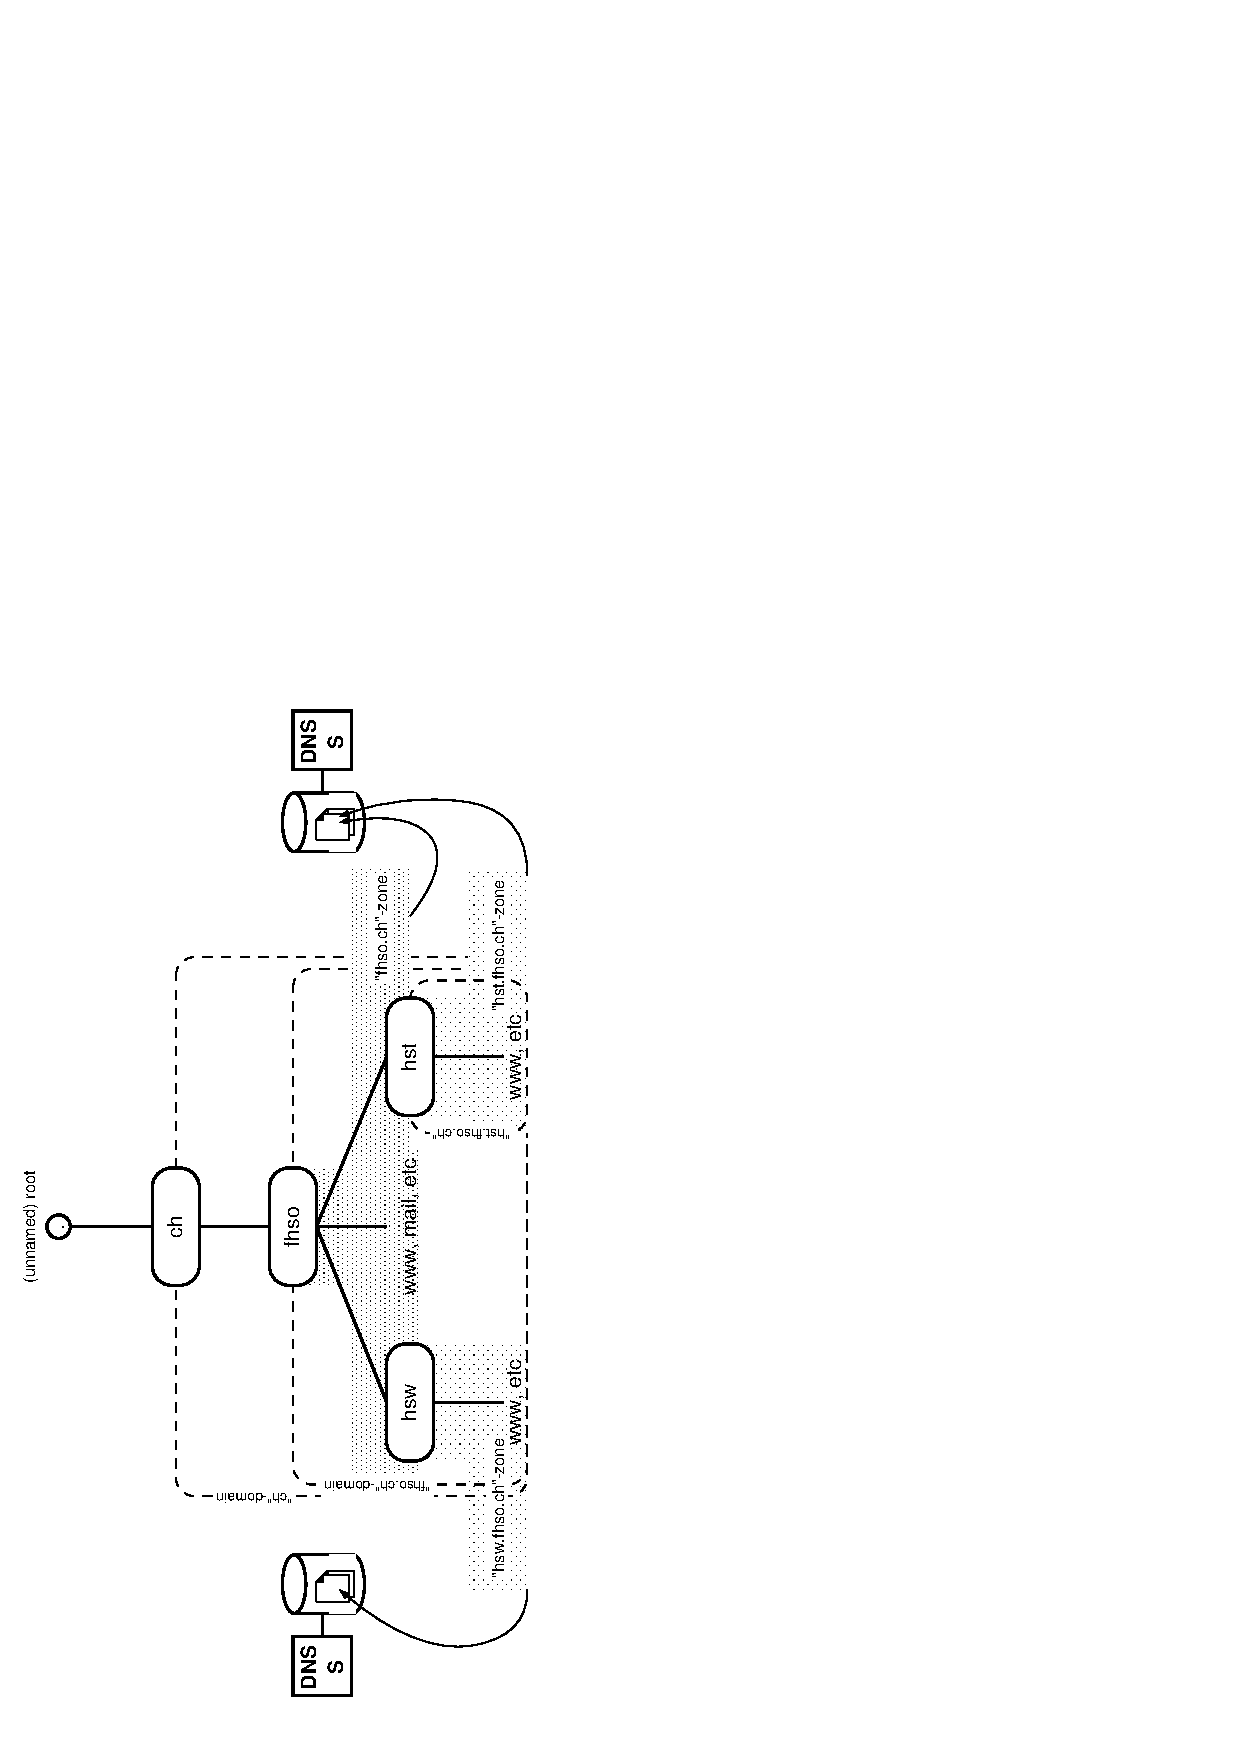
\includegraphics[height=8cm]{dns-serverhierarchy}\end{center}
\end{frame}




\begin{frame}
\frametitle{DNS: Verzeichniseintr\"age, \texttt{Key [Type] Value}}
\begin{itemize}
	\item{schlage \texttt{Key} im Verzeichnis nach und finde zugeh\"orige \texttt{Value}s}
	\item{{\em alle} Knoten (=\texttt{Key}) in der Verzeichnishierarchie haben zugeh\"orige \texttt{Value}s -- sonst w\"urden sie nicht existieren}
	\item{die Paarung \texttt{Type Value} wird als {\em resource-record} (RR) bezeichnet \begin{tiny}(vergleichbar mit Telefonbuch: zu einem Namen gibt es den Datentyp ``Telefonnummer''und den Inhalt ``0318921122'')\end{tiny}}
\end{itemize}
\begin{center}
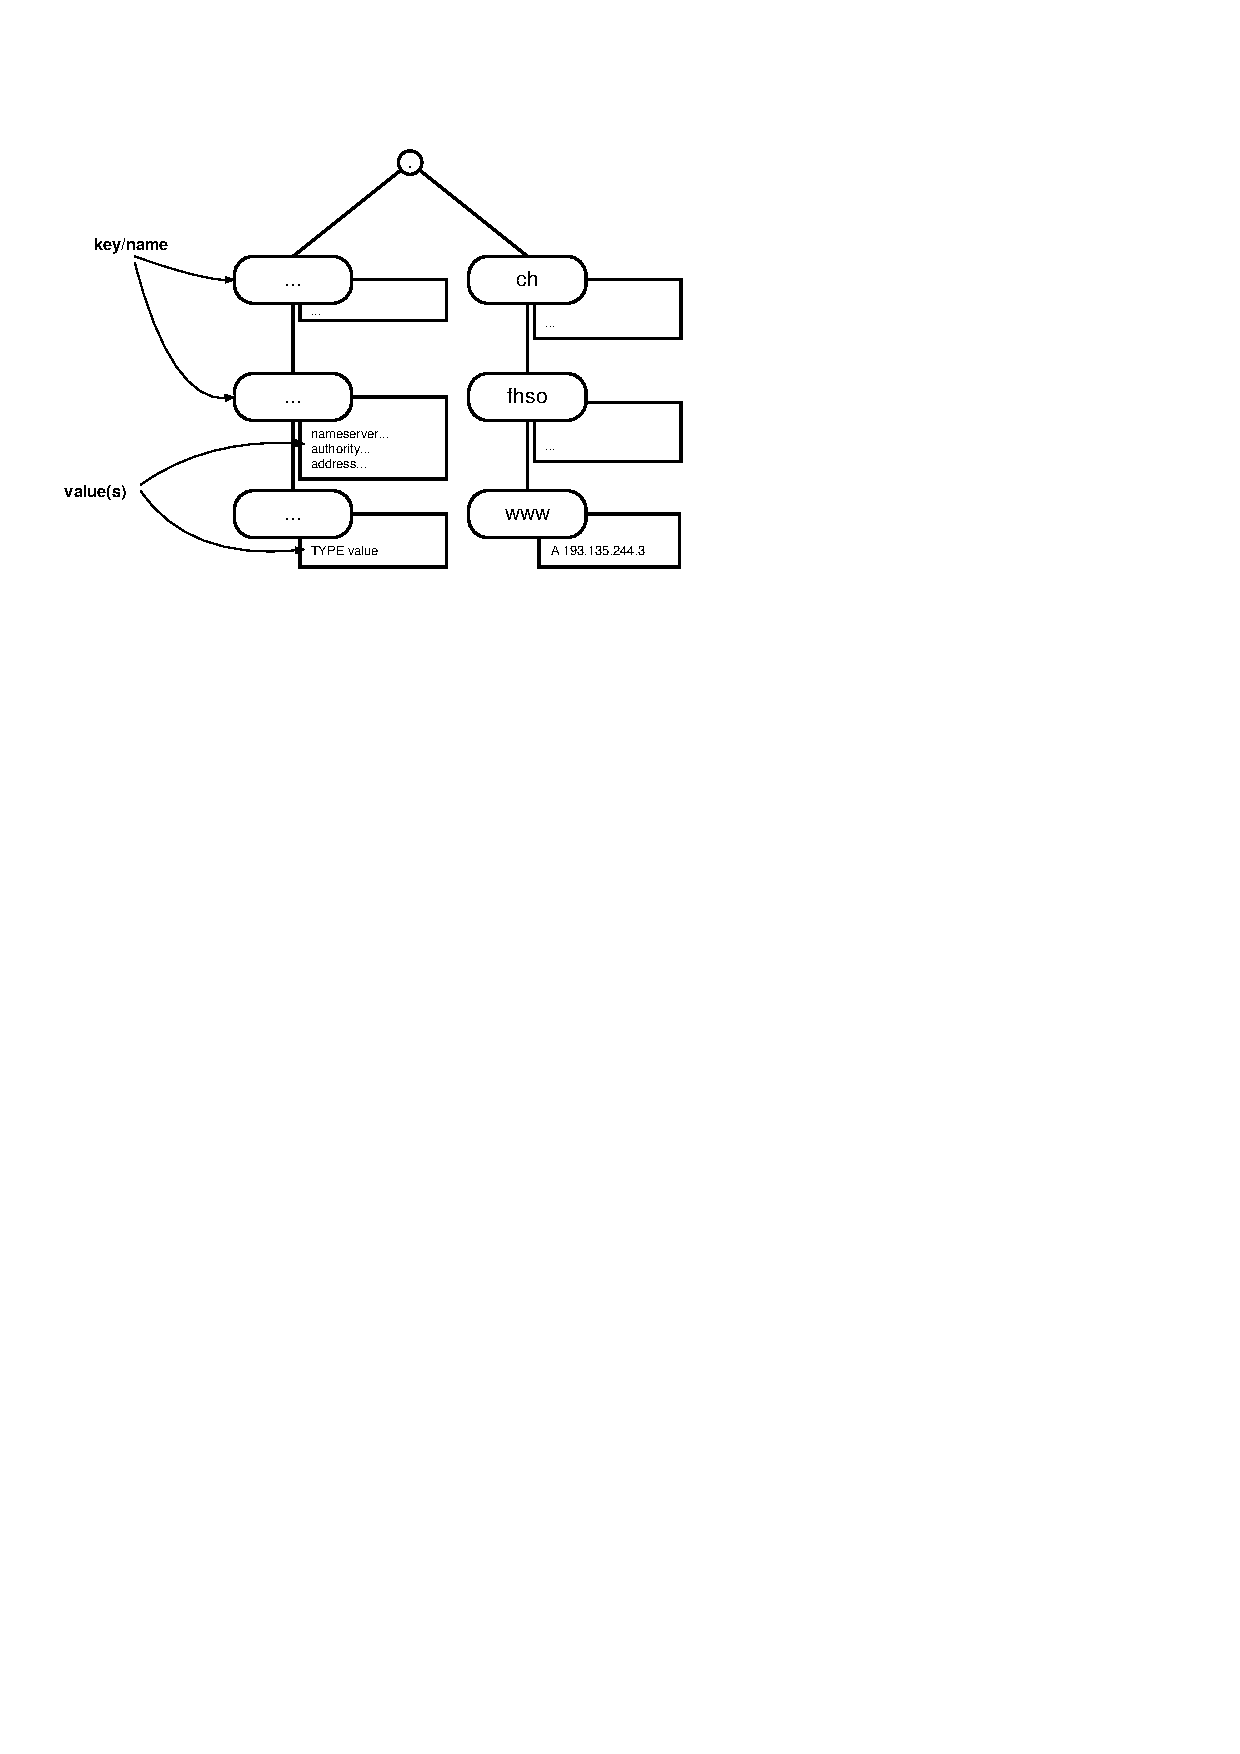
\includegraphics[width=12cm]{dns-keyvalue}
\end{center}
\end{frame}



\begin{frame}
\frametitle{DNS: Resource Records 1/2}
\hspace{-0.25cm}
\begin{small}
  \begin{tabular}{|c|l|l|}
  \hline
  RR-Type & Description & Syntax \\
  \hline
  \hline
  A & {\bf A}ddress: name $\rightarrow$ IP-address & {\tt {\em name} A {\em ip-address}} \\
  \hline
  PTR & {\bf P}oin{\bf t}e{\bf r}: IP-address $\rightarrow$ name & {\tt {\em rev-ip-name} PTR {\em name}} \\
  \hline
  SOA & {\bf S}tart-{\bf O}f-{\bf A}uthority: zone-head & 
  \begin{minipage}{8cm}{\tt {\em domain} SOA {\em origin} {\em mail} {\em (\\
      {\em serial}\\
      {\em refresh}\\
      {\em retry}\\
      {\em expiration}\\
      {\em minimum-TTL}\\
      )}}\end{minipage} \\
      \hline
      NS & {\bf N}ame {\bf S}erver & {\tt {\em domain} NS {\em name-of-ns}} \\
      \hline
      MX & {\bf M}ail E{\bf x}change: mail-server & {\tt {\em name} MX {\em priority} {\em name-of-mailserver}} \\
      \hline
      CNAME & {\bf C}anonical {\bf Name}: alias-name & {\tt {\em alias} CNAME {\em original}} \\
      \hline
      \ldots & \ldots & \ldots \\
      \hline
\end{tabular}
\end{small}
\end{frame}





\begin{frame}
\frametitle{DNS: Resource Records 2/2}
\begin{itemize}
	\item{\texttt{SOA}: jede Zone (Verzeichnisebene) muss einen solchen Record haben. Darin werden Verwaltungsdaten (Seriennummer, Abfrageintervall f\"ur {\em Slave}-Server, etc abgelegt}
	\item{\texttt{NS}: {\em Delegation}: zeigt auf den zust\"andigen Nameserver f\"ur die Zone in \texttt{Key}}
	\item{\texttt{A}: der ``normale'' Eintrag: \texttt{Key}=Name und \texttt{Value}=IP-Adresse}
	\item{\texttt{PTR}: der ``reverse'' Eintrag: IP-Adresse auf Namen}
	\item{\texttt{CNAME}: ein Alias-Name der \"ublicherweise f\"ur {\em Dienste} (versus Host/Server) verwendet wird}
	\item{\texttt{MX}: Mailserver f\"ur eine Domain}
	\item{das \texttt{TTL}-Feld bezeichnet f\"ur jeden RR die Lebensdauer als Cache-Inhalt}
	\item{es k\"onnen mehrere \texttt{Values} eines \texttt{Type}s f\"ur einen \texttt{Key} definiert werden}
\end{itemize}
\end{frame}




\begin{frame}
\frametitle{DNS: Tools}
normalerweise werden DNS-Abfragen durch das Betriebssystem\footnote{genauer: durch \texttt{gethostbyname()}} automatisch erledigt$\ldots$

zur manuellen Abfrage des DNS-Dienstes gibt es einige Kommandozeilenwerkzeuge\footnote{auf den meisten Betriebssystemen finden Sie auch GUI-Tools oder Sie benutzen: \myurl{http://www.dnsstuff.com/}}:
\begin{itemize}
	\item{\texttt{nslookup}: der ``Urvater''\\ \texttt{nslookup [-q={\em Type}] {\em Key} [{\em nameserver-to-use}]}}\\ oder einfach\\ \texttt{nslookup\\set type={\em Type}\\{\em Key}} (interaktiver Modus)
	\item{\texttt{host}: moderner Nachfolger von \texttt{nslookup} (UNIX):\\ \texttt{host [-t {\em Type}] {\em Key} [{\em nameserver-to-use}]}}
	\item{\texttt{dig} ist ein weiterer Nameserver-Client (UNIX)}
\end{itemize}
\end{frame}


\begin{frame}
\frametitle{DNS: Interlude}
\begin{itemize}
  \item{finden Sie die IP-Adresse von www.fhnw.ch}
  \item{finden Sie den Namen von 64.147.188.3 (versuchen Sie auch explizit \texttt{Type=PTR}}
  \item{finden Sie die Mailserver von kyoto-u.ac.jp, microsoft.com und apple.com}
	\item{finden Sie die Nameserver von ``.'' (root nameservers)}
	\item{finden Sie die Nameserver (DNS-Server) f\"ur mit.edu}
	\item{finden Sie den ``echten'' Namen von www.netlabs.ch und von postoffice.netlabs.ch}
\end{itemize}
\end{frame}


\begin{frame}
\frametitle{DNS: Server Rollen}
ein Nameserver kann verschiedene Rollen annehmen (auch gleichzeitig)
\begin{itemize}
	\item{Authoritative: der Server ist in den NS records angegeben und hat die Zonendaten lokal (Datei, DB) gespeichert. Antworten werden mit dem ``aa'' (authoritative-answer) bezeichnet}
	\item{Forwarding/Caching: der Server erledigt ``recursive-queries''\footnote{Slide \ref{recursive-query}} f\"ur Clients\footnote{f\"ur die Anfrage auf andere Nameserver nimmt er dann die Client-Rolle an} -- er ist nicht {\em authoritative} f\"ur die angefragten Daten. Typischerweise finden Sie forwarding-servers in Organisationen oder Providern f\"ur ``interne'' Clients}. Die Antworten werden auf dem caching-server zwischengespeichert
\end{itemize}
\begin{block}{Beispiel: dns.fhnw.ch}
Authoritative: f\"ur \texttt{fhnw.ch}\\
Caching/Forwarding: f\"ur alles andere
\end{block}
\end{frame}


\begin{frame}
\frametitle{DNS: Server-Replikation}
\begin{itemize}
  \item{in der Server-Konfiguration \em{f\"ur eine Zone} wird
    \begin{itemize}
      \item{ein \em{master}-Server\footnote{fr\"uher ``primary'' und ``secondary''}}
      \item{0 bis viele \em{slave}-Server}
    \end{itemize}
    definiert. Diese werden als \texttt{NS}-records f\"ur die Zone erfasst}
  \item{von ``aussen'' ist diese Rollenverteilung unwichtig/nicht eindeutig feststellbar\footnote{das entsprechende Informationsfeld im \texttt{SOA}-Record ist nur ``informativ''}: alle \texttt{NS}-Server sind gleichberechtigt (authoritative)}
  \item{die Replikation/Informationsabgleich kann auf zwei Arten gel\"ost werden:
    \begin{itemize}
      \item{im \texttt{SOA}-Record der Zone wird das Zeitintervall f\"ur ``Neuigkeiten''-Abfrage slave$\rightarrow$master festgelegt\footnote{\"uber das Versions-Feld im \texttt{SOA}-Record} wird eine \"Anderung festgestellt $\rightarrow$ ``polling''}
      \item{bei \"Anderungen der Daten auf dem master-Server werden die slave-Server mit einer speziellen Nachricht informiert $\rightarrow$ ``event triggered''}
     \end{itemize}}
   \item{in beiden F\"allen l\"auft die Synchronisation normalerweise \"uber TCP}
\end{itemize}
\end{frame}


\begin{frame}
\frametitle{DNS: Clients}
\begin{itemize}
	\item{Clients benutzen eine der Funktionen \texttt{gethostbyname}, \texttt{gethostbyaddr} oder \texttt{getaddrinfo} in den System-Bibliotheken\footnote{Library: \texttt{libc} oder \texttt{net}} um DNS-Abfragen zu senden}
	\item{moderne Betriebssysteme benutzen einen {\em lokalen} Cache-Dienst (\texttt{nscd}, ein eigener Prozess) um Anfragen von verschiedenen Prozessen/Programmen effizient zu verwalten (mit internem cacheing)}
	\item{\texttt{nslookup}, \texttt{host}, etc benutzen im Normalfall {\em nicht} diese Library}
	\item{zur korrekten Funktion muss mindestens ein Forwarding/Caching-Nameserver pro Client definiert werden (\texttt{/etc/resolv.conf}). Das passiert normalerweise \"uber DHCP}
	\item{mit dem \texttt{AA}-Flag\footnote{``AuthoritativeAnswer''} in der Antwort des Servers kann festgestellt werden ob die Antwort gecacht oder authoritative war}
\end{itemize}
\end{frame}



\begin{frame}\label{recursive-query}
\frametitle{DNS: Recursive Query}
\begin{itemize}
	\item{ein Client kann eine ``recursive query'' an einen Server stellen, der dann die ganze ``Arbeit'' \"ubernimmt und nur das Endergebnis liefert}
	\item{\begin{tiny}dazu muss der Client das ``rd'' recursion-desired flag setzten und der Server ``ra'' recursion-available anbieten\end{tiny}}
	\item{\begin{tiny}meistens wird vom Server ``ra'' nur an {\em interne} Clients angeboten\end{tiny}}
	\item ``Caching''-Server ist eine spezielle Rolle, die Queries weiterleiten (recursive) und lokal zwischenspeichern. Gleiche Anfragen werden aus dem Cache bedient
	\end{itemize}
\hspace{-0.5cm}\vspace{-1cm}
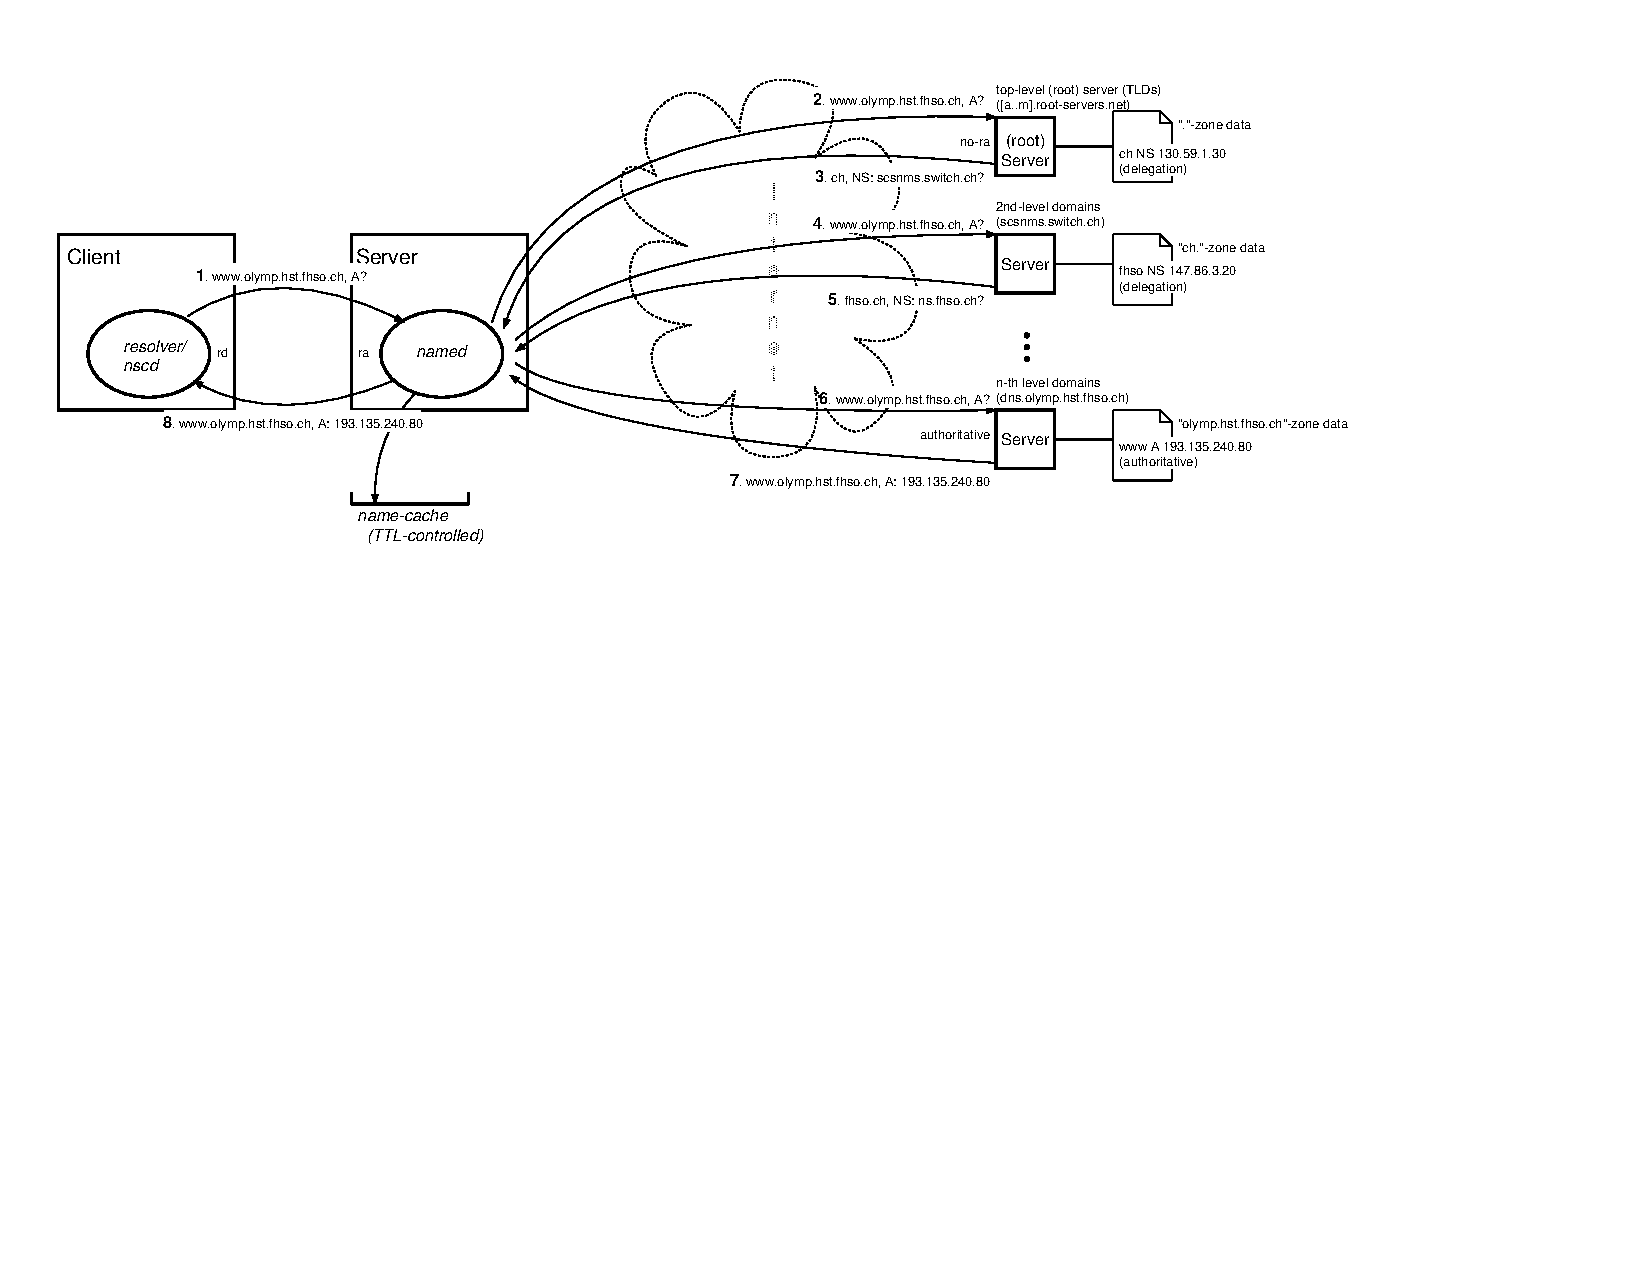
\includegraphics[width=15cm]{dns-recursive}
\end{frame}


\begin{frame}\label{caching}
\frametitle{DNS: Caching}
\begin{itemize}
	\item anders als z.B. bei ARP ist das Caching bei DNS \"uber den Parameter -- TTL\footnote{Time-To-Live, hier tats\"achlich eine Zeitangabe in Sekunden} -- genau geregelt
	\item TTL gibt an, wielange ein Caching-Server\footnote{oder ein Client-seitiger Cache} die zwischengespeicherte Antwort weiter ausliefern darf. Bei abgelaufener
	TTL muss der Authoritative-Server neu angefragt werden
	\item wenn eine Antwort aus einem Cache\footnote{oder generell von einem nicht-Authoritativen-Server} ausgeliefert wird, wird in der Antwort das ``AA'' (authoritative-answer) Flag {\em nicht} gesetzt
	\item eine lange\footnote{oft bei top-level Domainserver, z.B. a.nic.ch zu finden um die Last gering zu halten} Zeitangabe -- z.B. mehrere Tage -- f\"uhrt bei \"Anderungen am Resource-Record zu Problemen weil viele Caching-Server und auch Clients noch die alte Antwort weiterverwenden
	\item eine kurze\footnote{oft bei Webseiten, etc zu finden} Zeitangabe (einige Sekunden) ist zwar flexibel f\"uhrt aber zu wesentlich mehr Anfragen auf den ``Authoritative''-Server
\end{itemize}
\end{frame}


\begin{frame}\label{loadbalancing}
\frametitle{DNS: Loadbalancing}
\begin{itemize}
	\item manchmal werden auf eine Anfrage mehrere Antworten\footnote{f\"ur einen Resource-Record-Type} geliefert -- entspricht ``mehrere Telfonnummern''
	\item der Client w\"ahlt eine\footnote{meistens die erste} der gleichwertige Antworten f\"ur weitere Kommunikation aus
	\item Server ``rotieren'' die Antworten bei jeder Auslieferung und erreichen so eine primitive Art des Loadbalancings\footnote{verteilen von Anfragen \"uber mehrere -- z.B. Web -- Server}
\end{itemize}
\end{frame}



\begin{frame}[fragile]
\label{exercises-2}
\frametitle{DNS: Praktische \"Ubungen}
finden Sie Beispiele von:
\begin{itemize}
  \item kurze TTL 
  \item lange TTL
  \item ``round-robin''-Loadbalancing/mehrere Antworten
  \item beobachten Sie den ``decay''/das Ablaufen der TTL bei Abfrage eines Caching-Servers (z.B. 1.1.1.1, 8.8.8.8, 9.9.9.9)
\end{itemize}
verwenden sie wenn m\"oglich die Authoritative-Server (ausser bei Caching-Frage):

\begin{small}
\begin{Verbatim}
# mit dig, der @-Parameter ist der anzufragende Host 
# (hier der NS von post.ch, d.h. der authoritative-nameserver
dig www.post.ch @dns1.post.ch

# oder mit host
host -h dns1.post.ch www.post.ch
\end{Verbatim}
\end{small}
\end{frame}


\begin{frame}\label{doh-dot}
\frametitle{DNS: \href{https://en.wikipedia.org/wiki/DNS_over_HTTPS}{DoH} und \href{https://en.wikipedia.org/wiki/DNS_over_TLS}{DoT}\footnote{DNS-over-HTTPS, DNS-over-TLS}}
Eine neuere Entwickung ist die Implementierung einer verschl\"usselten Kommunikation (``privacy'') bei DNS-Abfragen
\begin{itemize}
  \item Caching-Server (z.B. die des Providers, des Campus) k\"onnen so nicht erkennen welche Abfragen gemacht werden (und auch nicht ver\"andern)
  \item die tats\"achliche IP-Kommunikation findet aber trotzdem vom Client zum Server statt -- die IP-Adressen sind wiederum ersichtlich
  \item der Benutzer vertraut einfach einem DoH/DoT-Betreiber\footnote{die auch ein Gesch\"aftsmodell haben\ldots} anstatt dem lokalen Providers, Campus, etc
\end{itemize}
\begin{block}{Kritik: Privacy ist auch ein Gesch\"aft}
Die DoT und DoH Server ``sehen'' nat\"urlich die Anfragen und k\"onnen daraus wichtige Meta/Statistik/Business-Daten erzeugen.
\\
Zudem gehen wichtige Sicherheitstechniken verloren (gesperrte Malware-Domains).
\end{block}
\end{frame}










\end{document}